% Which counters of the random state (k, c) the draws in a sub-graph use, and
% where the next draw after it continues: nv_scan() gives step i the counters
% after i bodies, nv_if() lets both branches continue the count and continues
% after the larger, nv_while() forks a child state whose counter the body
% advances, and the function gradient() differentiates continues the count like
% straight-line code.
% Build: see figures/README.md
\documentclass[tikz, border = 6pt]{standalone}
\usepackage[T1]{fontenc}
\usepackage{lmodern}
\usepackage{amsmath}
\usetikzlibrary{positioning, calc, arrows.meta, fit, backgrounds}

\definecolor{hash}{HTML}{5B8C5A}
\definecolor{keep}{HTML}{2A7AB0}
\definecolor{fork}{HTML}{E08A2C}
\definecolor{alt}{HTML}{8E6BB8}

\tikzset{
  >={Stealth[length = 2mm]},
  title/.style = {font = \ttfamily\small, anchor = west},
  sub/.style = {font = \footnotesize, text = black!60, anchor = west, align = left},
  cell/.style = {draw = black!45, minimum width = 1.25cm, minimum height = 6mm,
    font = \footnotesize, inner sep = 0pt},
  used/.style = {cell, fill = hash!20},
  usedb/.style = {cell, fill = keep!20},
  usedc/.style = {cell, fill = alt!20},
  spare/.style = {cell, fill = black!5, text = black!40},
  forked/.style = {cell, fill = fork!25},
  next/.style = {cell, draw = black!70, very thick, fill = white},
  brace/.style = {decorate, black!55},
  lab/.style = {font = \footnotesize, text = black!65},
  edge/.style = {->, black!60}
}
\usetikzlibrary{decorations.pathreplacing}

\begin{document}
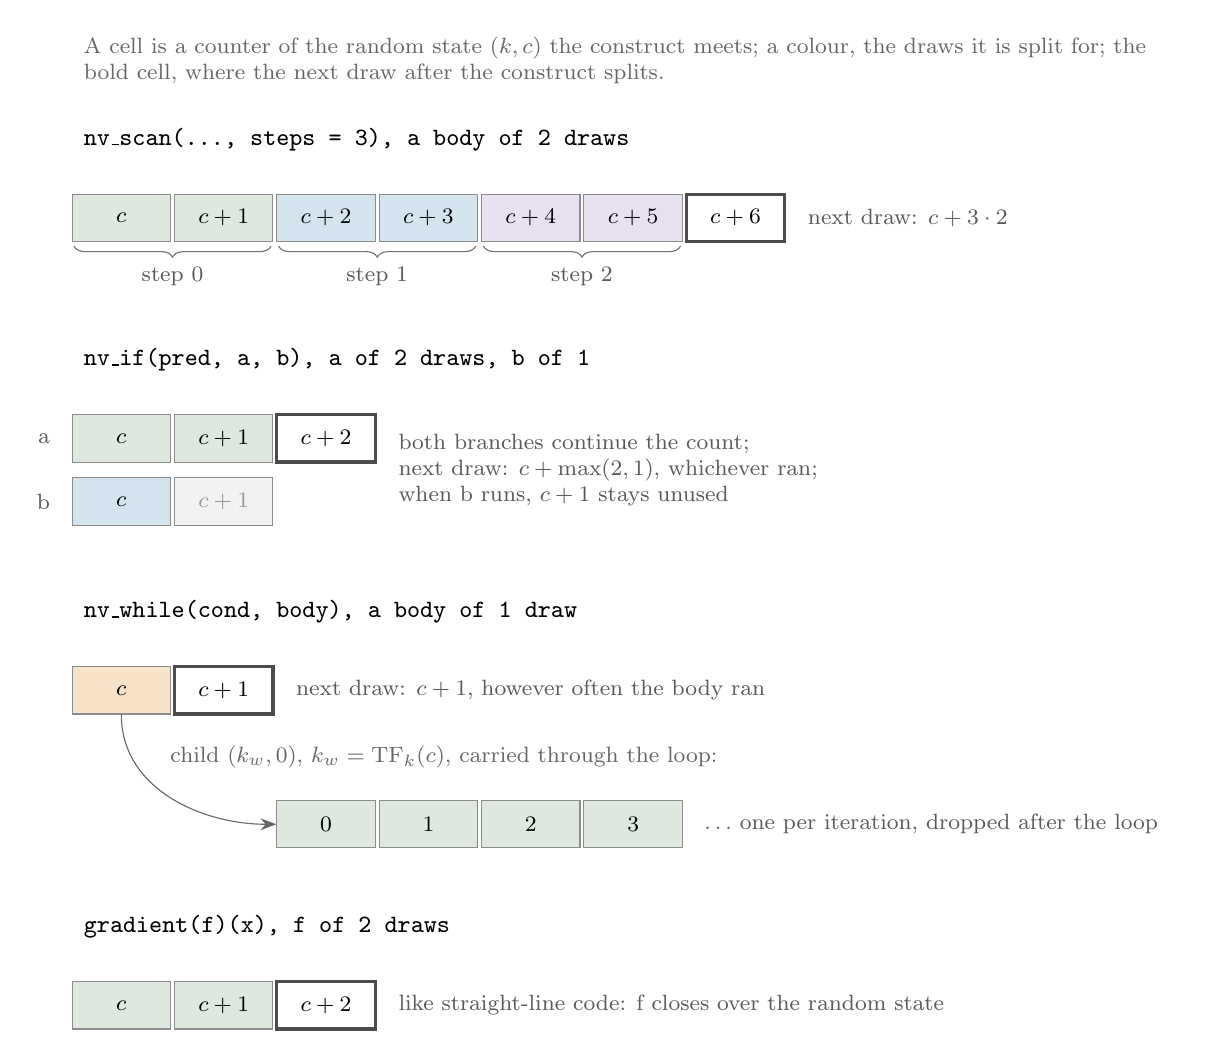
\begin{tikzpicture}

  \node[sub, text width = 14cm] at (-0.6, 2.0)
    {A cell is a counter of the random state $(k, c)$ the construct meets; a
     colour, the draws it is split for; the bold cell, where the next draw after
     the construct splits.};
  % ---- nv_scan ---------------------------------------------------------------
  \node[title] at (-0.6, 1.0) {nv\_scan(..., steps = 3), a body of 2 draws};
  \foreach \i/\style/\txt in {0/used/c, 1/used/c+1, 2/usedb/c+2, 3/usedb/c+3,
                              4/usedc/c+4, 5/usedc/c+5, 6/next/c+6} {
    \node[\style] (s\i) at (1.3 * \i, 0) {$\txt$};
  }
  \foreach \a/\b/\t in {0/1/step 0, 2/3/step 1, 4/5/step 2} {
    \draw[brace, decoration = {brace, mirror, amplitude = 4pt}]
      ($(s\a.south west) + (0.03, -0.05)$) -- ($(s\b.south east) + (-0.03, -0.05)$)
      node[lab, midway, below = 4pt] {\t};
  }
  \node[lab, anchor = west] at ($(s6.east) + (0.15, 0)$) {next draw: $c + 3 \cdot 2$};

  % ---- nv_if -----------------------------------------------------------------
  \node[title] at (-0.6, -1.8) {nv\_if(pred, a, b), a of 2 draws, b of 1};
  \foreach \i/\style/\txt in {0/used/c, 1/used/c+1, 2/next/c+2} {
    \node[\style] (a\i) at (1.3 * \i, -2.8) {$\txt$};
  }
  \foreach \i/\style/\txt in {0/usedb/c, 1/spare/c+1} {
    \node[\style] (b\i) at (1.3 * \i, -3.6) {$\txt$};
  }
  \node[lab, anchor = east] at ($(a0.west) + (-0.15, 0)$) {a};
  \node[lab, anchor = east] at ($(b0.west) + (-0.15, 0)$) {b};
  \node[lab, anchor = west, align = left] at ($(a2.east) + (0.15, -0.4)$)
    {both branches continue the count;\\next draw: $c + \max(2, 1)$, whichever ran;\\
     when b runs, $c + 1$ stays unused};

  % ---- nv_while --------------------------------------------------------------
  \node[title] at (-0.6, -5.0) {nv\_while(cond, body), a body of 1 draw};
  \foreach \i/\style/\txt in {0/forked/c, 1/next/c+1} {
    \node[\style] (w\i) at (1.3 * \i, -6.0) {$\txt$};
  }
  \node[lab, anchor = west] at ($(w1.east) + (0.15, 0)$)
    {next draw: $c + 1$, however often the body ran};
  \node[sub] at (0.5, -6.85) {child $(k_w, 0)$, $k_w = \mathrm{TF}_k(c)$, carried through the loop:};
  \foreach \i/\txt in {0/0, 1/1, 2/2, 3/3} {
    \node[used] (cw\i) at (1.3 * \i + 2.6, -7.7) {$\txt$};
  }
  \node[lab, anchor = west] at ($(cw3.east) + (0.15, 0)$) {$\ldots$ one per iteration, dropped after the loop};
  \draw[edge] (w0.south) to[out = -90, in = 180] (cw0.west);

  % ---- gradient --------------------------------------------------------------
  \node[title] at (-0.6, -9.0) {gradient(f)(x), f of 2 draws};
  \foreach \i/\style/\txt in {0/used/c, 1/used/c+1, 2/next/c+2} {
    \node[\style] (g\i) at (1.3 * \i, -10.0) {$\txt$};
  }
  \node[lab, anchor = west] at ($(g2.east) + (0.15, 0)$)
    {like straight-line code: f closes over the random state};

\end{tikzpicture}
\end{document}
